\documentclass[spanish,a4paper,11pt,twoside]{report}

%%%%%%%%%%%%%%%%%%%%%%%%%%%%%%%%%%%%%%%%%%%%%%%%%%%%%%%%%%%%%%%%%%%%%%%%%%%%%%%
\usepackage[dvips]{graphicx}
\usepackage[dvips]{epsfig}
\usepackage[latin1]{inputenc}
\usepackage[spanish]{babel}
\usepackage{alltt}
\usepackage{templates/algorithm}
\usepackage{templates/algorithmic}
\usepackage{templates/multirow}
\usepackage{amssymb}
%%%%%%%%%%%%%%%%%%%%%%%%%%%%%%%%%%%%%%%%%%%%%%%%%%%%%%%%%%%%%%%%%%%%%%%%%%%%%%%

\newcommand{\SONY}{{\sc Sony}}
\newcommand{\MICROSOFT}{{\sc Microsoft}}
\newcommand{\GCC}{\textsf{\textsc{G}CC}}
\newcommand{\INTEL}{\textsf{\textsc{I}ntel}}

\newcommand{\LAl}{{\lambda}}
\newcommand{\NA}{{$\mathbb{N}$}}

\newcommand{\LA}{{$\lambda$}}
\newcommand{\PHI}{{$\varphi$}}

%%% Traducimos el pseudocodigo
\renewcommand{\algorithmicwhile}{\textbf{mientras}}
\renewcommand{\algorithmicend}{\textbf{fin}}
\renewcommand{\algorithmicdo}{\textbf{hacer}}
\renewcommand{\algorithmicif}{\textbf{si}}
\renewcommand{\algorithmicthen}{\textbf{entonces}}
\renewcommand{\algorithmicrepeat}{\textbf{repetir}}
\renewcommand{\algorithmicuntil}{\textbf{hasta que}}
\renewcommand{\algorithmicelse}{\textbf{en otro caso}}
\renewcommand{\algorithmicfor}{\textbf{para}}

%\newcommand{\RETURN}{\textbf{retornar} }
\newcommand{\RET}{\STATE \textbf{retornar} }
\newcommand{\TO}{\textbf{hasta} }
\newcommand{\AND}{\textbf{y} }
\newcommand{\OR}{\textbf{o} }

%%%%%%%%%%%%%%%%% Creamos un entorno para listar c�digo fuente %%%%%%%%%%%%%%%
\newenvironment{sourcecode}
{\begin{list}{}{\setlength{\leftmargin}{1em}}\item\scriptsize\bfseries}
{\end{list}}

\newenvironment{littlesourcecode}
{\begin{list}{}{\setlength{\leftmargin}{1em}}\item\tiny\bfseries}
{\end{list}}

\newenvironment{summary}
{\par\noindent\begin{center}\textbf{Abstract}\end{center}\begin{itshape}\par\noindent}
{\end{itshape}}

\newenvironment{keywords}
{\begin{list}{}{\setlength{\leftmargin}{1em}}\item[\hskip\labelsep \bfseries Keywords:]}
{\end{list}}

\newenvironment{palabrasClave}
{\begin{list}{}{\setlength{\leftmargin}{1em}}\item[\hskip\labelsep \bfseries Palabras clave:]}
{\end{list}}


%%%%%%%%%%%%%%%%%%%%%%%%%%%%%%%%%%%%%%%%%%%%%%%%%%%%%%%%%%%%%%%%%%%%%%%%%%%%%%%
% Format
%%%%%%%%%%%%%%%%%%%%%%%%%%%%%%%%%%%%%%%%%%%%%%%%%%%%%%%%%%%%%%%%%%%%%%%%%%%%%%%

%%\topmargin -4 mm
%\topmargin -21 mm
%\headheight 10 mm
%\headsep 10 mm

%\textheight 229 mm
%\textheight 246 mm

%\oddsidemargin -5.4 mm
%\evensidemargin -5.4 mm
\oddsidemargin 5 mm
\evensidemargin 5 mm

%\oddsidemargin -3 mm
%\evensidemargin -3 mm

%\textwidth 17 cm
\textwidth 15 cm
%\columnsep 10 mm

\input{amssym.def}

%%%%%%%%%%%%%%%%%%%%%%%%%%%%%%%%%%%%%%%%%%%%%%%%%%%%%%%%%%%%%%%%%%%%%%%%%%%%%%%

\begin{document}

%%%%%%%%%%%%%%%%%%%%%%%%%%%%%%%%%%%%%%%%%%%%%%%%%%%%%%%%%%%%%%%%%%%%%%%%%%%%%%%
% First Page 
%%%%%%%%%%%%%%%%%%%%%%%%%%%%%%%%%%%%%%%%%%%%%%%%%%%%%%%%%%%%%%%%%%%%%%%%%%%%%%%

\pagestyle{empty}
\thispagestyle{empty}


\newcommand{\HRule}{\rule{\linewidth}{1mm}}
\setlength{\parindent}{0mm}
\setlength{\parskip}{0mm}
\vspace*{\stretch{1}}

\begin{center}

\includegraphics[width=0.2\textwidth]{images/logotipo-secundario-ULL}\\[0.25cm]
\end{center}

\HRule
\begin{center}
        {\Huge Distribuci�n de Poisson} \\[2.5mm] 
%        {\Huge Subt�tulo} \\[2.5mm]
	{\Large Alba Tom� Rodr�guez} \\[2mm]
	{\Large D�cil Batista Garc�a} \\[2mm]
	{\Large Desire� Praena Pacheco} \\[5mm]
%        {\Large Alba Tom� Rodr�guez\\D�cil Batista Garc�a\\Desir� Praena Pacheco} \\[5mm]
        {\Large \textit{Grupo ($3D$) }} \\[5mm]


        {\em T�cnicas Experimentales. $1^{er}$ curso. $2^{do}$ semestre} \\[5mm]
        Lenguajes y Sistemas Inform�ticos \\[5mm]
        Facultad de Matem�ticas \\[5mm]
        
        Universidad de La Laguna \\
\end{center}
\HRule
\vspace*{\stretch{2}}
\begin{center}
  La Laguna, \today 
\end{center}

%%%%%%%%%%%%%%%%%%%%%%%%%%%%%%%%%%%%%%%%%%%%%%%%%%%%%%%%%%%%%%%%%%%%%%%%%%%%%%%

%%%%%%%%%%%%%%%%%%%%%%%%%%%%%%%%%%%%%%%%%%%%%%%%%%%%%%%%%%%%%%%%%%%%%%%%%%%%%%%
\newpage{\pagestyle{empty}\cleardoublepage}

\pagestyle{myheadings} %my head defined by markboth or markright
% No funciona bien \markboth sin "twoside" en \documentclass, pero al
% ponerlo se dan un mont�n de errores de underfull \vbox, con lo que no se
% ha puesto.
\markboth{Alba, D�cil, Desire�}{Distribuci�n de Poisson}

%%%%%%%%%%%%%%%%%%%%%%%%%%%%%%%%%%%%%%%%%%%%%%%%%%%%%%%%%%%%%%%%%%%%%%%%%%%%%%%
%Numeracion en romanos
\renewcommand{\thepage}{\roman{page}}
\setcounter{page}{1}

%%%%%%%%%%%%%%%%%%%%%%%%%%%%%%%%%%%%%%%%%%%%%%%%%%%%%%%%%%%%%%%%%%%%%%%%%%%%%%%

\tableofcontents

%%%%%%%%%%%%%%%%%%%%%%%%%%%%%%%%%%%%%%%%%%%%%%%%%%%%%%%%%%%%%%%%%%%%%%%%%%%%%%%
\newpage{\pagestyle{empty}\cleardoublepage}

\listoffigures

%%%%%%%%%%%%%%%%%%%%%%%%%%%%%%%%%%%%%%%%%%%%%%%%%%%%%%%%%%%%%%%%%%%%%%%%%%%%%%%
\newpage{\pagestyle{empty}\cleardoublepage}

\listoftables

%%%%%%%%%%%%%%%%%%%%%%%%%%%%%%%%%%%%%%%%%%%%%%%%%%%%%%%%%%%%%%%%%%%%%%%%%%%%%%%
\newpage{\pagestyle{empty}\cleardoublepage}

%%%%%%%%%%%%%%%%%%%%%%%%%%%%%%%%%%%%%%%%%%%%%%%%%%%%%%%%%%%%%%%%%%%%%%%%%%%%%%%
%Numeracion a partir del capitulo I
\renewcommand{\thepage}{\arabic{page}}
\setcounter{page}{1}

\setlength{\parindent}{5mm}


%%%%%%%%%%%%%%%%%%%%%%%%%%%%%%%%%%%%%%%%%%%%%%%%%%%%%%%%%%%%%%%%%%%%%%%%%%%%%%%
\begin{abstract}

\\
El presente informe recoge informaci�n sobre la distribuci�n de Poisson. En �l se muestran definiciones fundamentales para la comprensi�n de �sta,as� como ejemplos, aplicaciones y el dise�o de un experimento en el cual se aplica dicha distribuci�n.

\\
De ella podemos decir que es una de las distribuciones m�s importantes de variable discreta (como la conocida binomial) pues los valores que puede tomar la variable aleatoria son n�meros naturales. Es muy �til cuando la muestra o segmento 'n' es grande y la probabilidad de �xitos 'p' es peque�a.

\\
La distribuci�n de Poisson se utiliza en situaciones donde los sucesos son impredecibles o de ocurrencia aleatoria. En otras palabras no se sabe el total de posibles resultados.

\end{abstract}
%%%%%%%%%%%%%%%%%%%%%%%%%%%%%%%%%%%%%%%%%%%%%%%%%%%%%%%%%%%%%%%%%%%%%%%%%%%%%%%
\chapter{Motivaci�n y objetivos}
\label{chapter:obj}

%%%%%%%%%%%%%%%%%%%%%%%%%%%%%%%%%%%%%%%%%%%%%%%%%%%%%%%%%%%%%%%%%%%%%%%%%%%%%
% Chapter 1: Motivaci�n y Objetivos 
%%%%%%%%%%%%%%%%%%%%%%%%%%%%%%%%%%%%%%%%%%%%%%%%%%%%%%%%%%%%%%%%%%%%%%%%%%%%%%%

En la vida cotidiana aparecen distintas situaciones que conviene analizar para realizar informes, estudios, predicciones, etc. Ejemplos de ellas podr�an ser el 'N�mero de hijos por pareja de un pa�s' o el 'N�mero de piezas defectuosas en un lote de 100 bombillas'. Dada la naturaleza de estas variables y considerando la definiciones que se muestran a lo largo del informe, se puede admitir que seguir�n una distribuci�n de Poisson.
\\
Por esto el objetivo principal de este trabajo va a ser la implementaci�n en Python de una distribuci�n de Poisson, para as� poder encontrar soluci�n a este tipo de problemas.


%%%%%%%%%%%%%%%%%%%%%%%%%%%%%%%%%%%%%%%%%%%%%%%%%%%%%%%%%%%%%%%%%%%%%%%%%%%%%%
\section{Ejemplo 1. Distribuci�n de los amino�cidos en las prote�nas}
\label{1:sec:1}
Antes del descubrimiento del c�digo gen�tico aceptado actualmente, se hab�an propuesto ciertos c�digos basados, entre otras, en consideraciones de dependencia entre los amino�cidos de una prote�na. ( C�digo Tri�ngulo y c�digo Diamante)
Una experiencia de Gamow parece indicar que no se dan tales relaciones, al menos para las prote�nas estudiadas. Se compilaron los dip�ptidos que pod�an formarse tomando amino�cidos vecinos, en una muestra de prote�nas con unas proporciones de amino�cidos bastante equilibradas, descartando algunas con una composici�n altamente especializada. Con la muestra utilizada pod�an formarse 177 dip�ptidos, de este tipo. Si se consideran 20 amino�cidos distintos, pueden formarse $20*20=400$ \ combinaciones diferentes de dos amino�cidos, con lo que, por t�rmino medio se observar�n:\\
\\
\centerline{ $\frac{177}{400}=0.442$} dip�ptidos de un tipo.\\
\\
Los 400 pares posibles pueden considerarse como ''casilla'', a las que un dip�ptido ''pertenece'' si est� formado por aquellos dos amino�cidos, pero se repite la experiencia un n�mero de veces $N=177$, grande (n�mero de dip�ptidos realmente observados), la variable aleatoria $x$= "n�mero de dip�ptidos en una casilla", seguir� una distribuci�n de Poisson\\
\\
\centerline {$f(x)= e^{-\LAl}\frac{\LAl^x}{x!}$  (x = 0,1,2,3,\dots,n,\dots)}\\
\\
siendo $\LAl=\frac{177}{400}=0.442$, de manera que el n�mero esperado de casillas con x dip�ptidos ser� $Nf(x)$.\\
\\
 Los resultados se resumen en la tabla anexa (v�ase el cuadro \ref {tabla1}). Como se puede apreciar en ella, la distribuci�n de dip�ptidos observada se ajusta en gran medida a la esperada seg�n la distribuci�n de Poisson, cosa que no ocurre con la distribuci�n esperada seg�n los c�digos ''Diamante'' y ''Triangulo''.

%--------------------------------------------------------------------------
\begin{table}[!ht]
\begin{center}
\begin{tabular}{|l|c|c|c|c|} \hline 

%Nº dipéptidos & Función observada & Código "Triángulo" & Código "Diamante" & Distribución de Poisson \\ 
N & F & CT & CD & D. Poisson\\ \hline
0 & 264 & 276 & 305 & 264.2 \\ \hline
1 & 103 & 86 & 55 & 116.0 \\ \hline
2 & 27 & 26 & 23 & 25.6 \\ \hline
3 & 4 & 9 & 7 & 3.77 \\ \hline
4 & 2 & 3 & 3 & 0.42 \\ \hline
5 & 0 & 0 & 3 & 0.037 \\ \hline
6 & 0 & 0 & 2 & 0.0027 \\ \hline
7 & 0 & 0 & 0 & $1.7x10^{-4}$\\ \hline
8 & 0 & 0 & 2 & $9.5x10^{-6}$ \\ \hline

\end{tabular}
\end{center}
\caption{Datos}
\label{tabla1}
\end{table}


%---------------------------------------------------------------------------------
\section{Ejemplo 2. Carnavales}
La probabilidad de que en carnavales una persona se desmaye es de 0.001. Considerando que acuden unas 5000 personas, �cu�l es la probabilidad de que se desmayen 25 personas?\\
\\
\large Soluci�n:\\
\\
Se trata de una binomial con $n=5000$ y $p=0.001$. La probabilidad ser�a:\\
\\
\centerline {$F(x=25)={5000 \choose 25}0.001^{25}(1-0.001)^{5000-25}$}\\
\\
que resulta complejo de calcular. Por eso se prefiere aproximar a una distribuci�n de Poisson, con \LA \ = $5000*0.001=50$, y quedar�a:\\
\\
\centerline {$F(x=25)=(e^{-50})\frac{50^{25}}{25!}=3.70*10^{-5}$}

%%%%%%%%%%%%%%%%%%%%%%%%%%%%%%%%%%%%%%%%%%%%%%%%%%%%%%%%%%%%%%%%%%%%%%%%%%%%%%%%%%%%

\section{Ejemplo 3. Cheques sin fondo}
Si un banco recibe en promedio 6 cheques sin fondo por d�a, �cu�les son las probabilidades de que reciba:\\
\begin{enumerate}
\item cuatro cheques sin fondo en un d�a dado?
\item diez cheques sin fondo en cualquiera de dos d�as consecutivos?
\end{enumerate}
\large Soluci�n:
\begin{enumerate}
\item x = variable que nos define el n�mero de cheques sin fondo que llegan al banco en un d�a cualquiera=0,1,2,3,\dots.
\LA \ = 6 cheques sin fondo por d�a.\\
\\
\centerline {$p(x=4,\LAl=6)= \frac{6^{4}2.718^{-6}}{4!} = \frac{(1296)(0.00248)}{24} = 0.13392$}
\item x = variable que nos define el n�mero de cheques sin fondo que llegan al banco en dos d�as consecutivos=0,1,2,3,\dots.
$\LAl \ =6*2=12 $ cheques sin fondo en promedio que llegan al banco en dos d�as consecutivos.\\
\\
\centerline {$p(x=10,\LAl=12)= \frac{12^{10}2718^{-12}}{10!} = \frac{(6.1917364*10^{10})(0.000006151)}{3628800} = 0.104953$}
\end{enumerate}



%%%%%%%%%%%%%%%%%%%%%%%%%%%%%%%%%%%%%%%%%%%%%%%%%%%%%%%%%%%%%%%%%%%%%%%%%%%%%%%
\chapter{Fundamentos te�ricos}
\label{chapter:teo}

%%%%%%%%%%%%%%%%%%%%%%%%%%%%%%%%%%%%%%%%%%%%%%%%%%%%%%%%%%%%%%%%%%%%%%%%%%%%%%%
% Chapter 2: Fundamentos Te�ricos 
%%%%%%%%%%%%%%%%%%%%%%%%%%%%%%%%%%%%%%%%%%%%%%%%%%%%%%%%%%%%%%%%%%%%%%%%%%%%%%%

%++++++++++++++++++++++++++++++++++++++++++++++++++++++++++++++++++++++++++++++

%++++++++++++++++++++++++++++++++++++++++++++++++++++++++++++++++++++++++++++++

\section{Historia de la Distribuci�n de Poisson}

\label{2:sec:1}
 

La distribuci�n fue introducida por primera vez por Sime�n Denis Poisson, f�sico y matem�tico franc�s al que se le conoce por sus diferentes trabajos en el campo de la electricidad y que tambi�n hizo publicaciones sobre la geometr�a diferencial y la teor�a de probabilidades, en la que nos centraremos. La distribuci�n fue publicada, junto con su teor�a de la probabilidad, en 1837 en su obra ''Recherches sur la probabilit des jugements en matire criminelle et en matire civile'', un trabajo importante en el cual describe la probabilidad como un acontecimiento fortuito ocurrido en un tiempo o intervalo bajo las condiciones siguintes: la probabilidad de que un acontecimiento ocurra es muy peque�a, pero el n�mero de intentos es muy grande. Entonces el evento ocurre algunas veces. El resultado hab�a sido dado previamente por Abraham de Moivre en ''De Mensura Sortis seu, de Probabilitate Eventuum en Ludis un Casu fortuito Pendentibus'' en Philosophical Transactions de la Royal Society, p. 219.
\\
\\
Una aplicaci�n pr�ctica de esta distribuci�n fue hecha por Ladislao Bortkiewicz en 1898 cuando se le dio la tarea de investigar el n�mero de soldados en el ej�rcito prusiano matados accidentalmente por tiro de caballos. Este experimento introdujo la distribuci�n de Poisson para el campo de la ingenier�a de confiabilidad. ( Ve�se la figura \ref{imagen})

\begin{figure}[!th]
\begin{center}
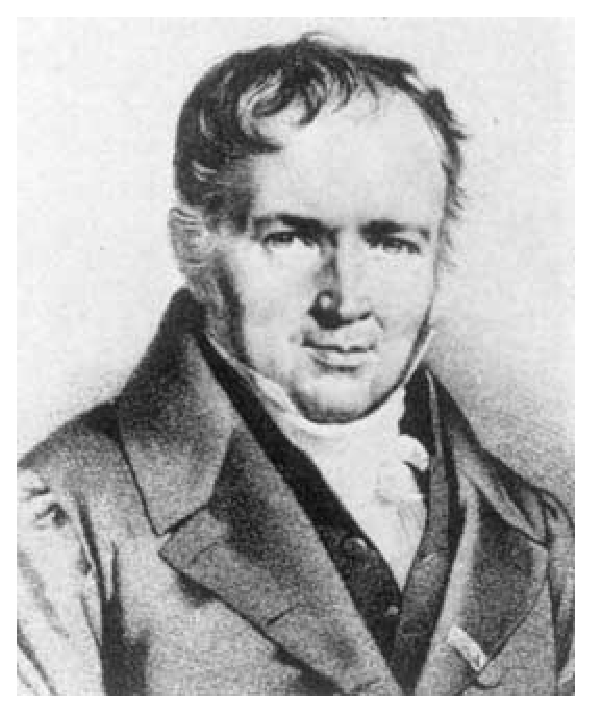
\includegraphics[width=0.25\textwidth]{images/Poisson.eps}
\caption{Sime�n Denis Poisson}
\label{imagen}
\end{center}
\end{figure}


%---------------------------------------------------------------------------------
\section{Conceptos fundamentales}

Para entender la distribuci�n de Poisson hemos de tener en cuenta conceptos fundamentales como por ejemplo:\\ 
\begin{itemize}
\item \textbf{Variable aleatoria:} En palabras simples, podemos decir que, dado un experimento aleatorio y asociado al mismo un espacio probabil�stico, una variable aleatoria es una aplicaci�n que a cada valor del espacio muestral le hace corresponder un n�mero real. Se clasifican en:\\
\begin{itemize}
\item \textbf{Discretas:} si los n�meros asociados a los sucesos son puntos aislados. Por ejemplo:\\
''Lanzar una moneda 3 veces y que salga cara''. Los posibles resultados son (0,1,2,3).
\item \textbf{Continuas:} los valores asignados pueden ser cualesquiera dentro de ciertos intervalos. Por ejemplo:\\
''Tomando la variable nivel de agua de un embalse'', pueden obtenerse valores entre $0$ y $\infty$.
\end{itemize}
\end{itemize}

%%%%%%%%%%%%%%%%%%%%%%%%%%%%%%%%%%%%%%%%%%%%%%%%%%%%%%%%%%%%%%%%%%%%%%%%%%%%%%%%%%%%

\subsection {Distribuci�n de Poisson}

Sea $X$ una variable aleatoria de una distribuci�n discreta definida sobre un espacio de probabilidad, se dice que $X$ tiene una distribuci�n de Poisson de par�metro \LA si su funci�n de densidad ( es decir, funci�n que describe el comportamiento probabil�stica de la variable) es:\\
\\
\centerline{$f(x)=\left\{
	\begin{array}{ll}
	P[X=x]=e^{- \LAl}\frac{\LAl^{x}}{x!} & \mathrm{,si\ } x \in \mathbb{N}  \\
	0 & \mathrm{,en\ otro\ caso\ } 
	\end{array}
\right.$} 
\\
\\
donde \LA \ es un par�metro caracter�stico de la distribuci�n. A dicha distribuci�n se denomina $P$(\LA).

%%%%%%%%%%%%%%%%%%%%%%%%%%%%%%%%%%%%%%%%%%%%%%%%%%%%%%%%%%%%%%%%%%%%%%%%%%%%%%%%%%%%%

\subsection {Aproximaci�n de la binomial a la Poisson}

La Poisson se puede obtener de la binomial en determinadas condiciones. Sea $X$ una variable aleatoria con distribuci�n binomial $B(n,p)$, cuya funci�n de densidad es:\\
\\
\centerline{$f(X)={n\choose k}p^k(1-p)^{n-k}$}\\
\\
Cuando el n�mero de pruebas $n \rightarrow \infty$ y la probabilidad del suceso tiende a cero y $np \rightarrow$ \LA \ entonces:\\
\\
\centerline{$\displaystyle\lim_{n \to{+}\infty\\ p \to 0\\ np \to \LAl}{f(x)}=e^{-\LAl}\frac{\LAl^k}{k!}$}\\
\\
que es la funci�n de distribuci�n de Poisson, es decir, $B(n,p)\rightarrow P$(\LA) bajo las condiciones anteriores.

%%%%%%%%%%%%%%%%%%%%%%%%%%%%%%%%%%%%%%%%%%%%%%%%%%%%%%%%%%%%%%%%%%%%%%%%%%%%%%%%%%%%%

\section{Propiedades}
\begin{enumerate}
\item \textbf{\large Esperanza}\\
\\
La media o esperanza matem�tica de $P$(\LA) es:\\
\\
\centerline {$E(X)=$\LA}

\item \textbf{\large Varianza}\\
\\
Respecto a la varianza,\\
\centerline {$Var(X)=\LAl=E(X)$}

\item \textbf{\large El par�metro \LA}\\
\\
El par�metro \LA \ de una distribuci�n de Poisson caracteriza a la misma:\\
\\
\centerline {\LA \ $ = \displaystyle\lim_{n \to{+}\infty\\ p \to 0}{np}$}
Se puede obtener de varias formas:\\
\begin{itemize}
\item $n$ y $p$ conocidas\\
\centerline {\LA \ $ = np$}
\item A partir de la esperanza\\
\centerline {\LA \ $ = E(X)$}
\item Estimando a partir de una muestra\\
\centerline {\LA \ $ = m( X_1,\dots,X_s) = \frac{1}{s}\displaystyle\sum_{i=1}^s X_i$} 
\item A partir de la probabilidad del suceso [$X=0$] ya que\\
\\
\centerline {$P[X=0] = f(0) = e^{-\LAl}\frac{\LAl^0}{0!} = e^{-\LAl}$}
luego \LA \ $ = -\ln P[X=0]$
\end{itemize}

\item \textbf{\large Funci�n caracter�stica}\\
\\
La funci�n caracter�stica viene dada por:\\
\\
\centerline {\PHI \ $ = e^{\LAl(e^{it}-1)}$}
\end{enumerate}
%%%%%%%%%%%%%%%%%%%%%%%%%%%%%%%%%%%%%%%%%%%%%%%%%%%%%%%%%%%%%%%%%%%%%%%%%%%%%%%%%%%%%
\section{Aplicaciones}
\begin{itemize}
\item Estimaci�n del n�mero de diferencias g�nicas entre dos especies a partir de datos sobre la identidad electrofor�tica de sus prote�nas.
\item Liberaci�n de cuantos de acetilcolina en las terminaciones nerviosas. ( Sigue $P$(\LA))
\item Consideraciones sobre las hip�tesis explicativas del proceso de extinci�n de 10 �rdenes de reptiles en el Cret�cico.
\item Distribuci�n de los amino�cidos en las prote�nas.
\item Contaje del n�mero de gl�bulos rojos en una muestra de sangre.
\end{itemize}


%\section{Segundo apartado del segundo cap�tulo}
%\label{2:sec:2}
%  Primer p�rrafo de la segunda secci�n.



%%%%%%%%%%%%%%%%%%%%%%%%%%%%%%%%%%%%%%%%%%%%%%%%%%%%%%%%%%%%%%%%%%%%%%%%%%%%%%%
\chapter{Procedimiento experimental}
\label{chapter:exp}

%%%%%%%%%%%%%%%%%%%%%%%%%%%%%%%%%%%%%%%%%%%%%%%%%%%%%%%%%%%%%%%%%%%%%%%%%%%%%%%
% Chapter 3: Procedimiento experimental 
%%%%%%%%%%%%%%%%%%%%%%%%%%%%%%%%%%%%%%%%%%%%%%%%%%%%%%%%%%%%%%%%%%%%%%%%%%%%%%%
El experimento realizado consiste en aproximar la distribuci�n de los amino�cidos en las prote�nas mediante la Poisson. (Ejemplo 1 del primer cap�tulo)
Adem�s, una vez obtenidos los datos, se podr�n comparar con experimentos realizados antes de la aparici�n del modelo de Poisson y con los datos reales observados.

%++++++++++++++++++++++++++++++++++++++++++++++++++++++++++++++++++++++++++++++
\section{Descripci�n de los experimentos}
\label{3:sec:1} 

Teniendo en cuenta la descripci�n dada en el Ejemplo 1, Cap�tulo 1 (Motivaci�n y objetivos), se ha dise�ado un modelo preparado para aplicar la distribuci�n de Poisson a un n�mero entero  'n', que ser� introducido por el usuario, y que representa el n�mero de dip�ptidos (uni�n de dos amino�cidos, estructuras principales de las prote�nas).
Adem�s, la funci�n de distribuci�n consta de un par�metro 'lambda' que es constante pero que hay que calcular en base a los datos dados del experimento.\\
En este caso,  se toma una muestra con la que podr�an formarse 177 dip�ptidos de un total de 400 combinaciones diferentes (por ser dip�ptidos -2- y haber 20 prote�nas posibles: 20x20=400), por tanto, nuestro par�metro ser� la cantidad constante 177/400 = 0.442 . \\
Una vez introducido el n�mero 'n', el algoritmo calcula la probabilidad de que exista una casilla con 'n' dip�ptidos, entendiendo por casilla  el total (400).
Posteriormente, muestra una tabla en la que aparecen, desde 0 hasta 'n' el n�mero de dip�ptidos, su probabilidad seg�n la distribuci�n y la frecuencia total (400x'n').
\\
\\
\\

El algoritmo es el siguiente:
\\
\begin{verbatim}
#!/usr/bin/python
#!encoding: UTF-8

import sys
import math

def calcular_poi(n):
  lam = 0.4425
  f_i=1 #factorial
  for i in range(n+1):
    if i==0:
      f_i=f_i
    else:
      f_i=f_i*i;
  ex = math.exp(-lam)
  ln = lam**n
  v1 = ex * ln
  valor_poi = v1 / f_i
  return (valor_poi)
    
#programa principal

argumentos = sys.argv[1:]

if (len(argumentos) == 1 ):
  n = int (argumentos[0]);
else:
  print 'Introduzca el n�mero de  dip�ptidos(0<n<10):'
  n = int (raw_input());
    
if (n>0):

  lista = [] #para indicar que es una variable de tipo lista
  for i in range (n+1):

    valor = calcular_poi(i)
    lista.append (valor) #para a�adir valores a la lista

  print "numero de dipeptidos por casilla\tdistribucion de Poisson (f(x))\t400xf(x)"
    
  for i in range (n+1):
    print "%d\t\t\t\t\t%1.10f\t\t\t%1.10f" % (i, lista[i],400*lista[i])
      
   
else:
  print 'el n�mero de dipeptidos debe ser mayor que 0'


\end{verbatim}

Este estudio se ha hecho para el n�mero de dip�ptidos 'n' = 8 , con lo que se solicita al usuario que el n�mero est� en el intervalo [0,10].
No obstante, el algoritmo es v�lido para n�meros naturales mayores.

En el Ap�ndice 1 se especifica el nombre del archivo de extensi�n Python que debe ejecutarse para realizar el experimento.

%++++++++++++++++++++++++++++++++++++++++++++++++++++++++++++++++++++++++++++++
\section{Descripci�n del material}
\label{3:sec:2}

Para la implementaci�n del algoritmo, como ya se ha mencionado en varias ocasiones, se ha utilizado Python.
\\
\\

Las caracter�sticas de la m�quina desde la que se ha realizado el informe son las siguientes:
\\
\\


('default', 'Feb 27 2014 20:00:17')\\
Linux-3.2.0-61-generic-i686-with-Ubuntu-12.04-precise\\
('Linux', 'PROA', '3.2.0-61-generic', '#93-Ubuntu SMP Fri May 2 21:33:33 UTC 2014', 'i686', 'i686')\\
2.7.3\\
Intel(R) Celeron(R) M CPU        520  @ 1.60GHz\\
GenuineIntel\\
1595.908 Hz\\
1024 KB\\
\\
\\

Adem�s, se ha estudiado el tiempo que tarda la m�quina en ejecutar el algoritmo principal en funci�n del dato introducido. Ver Figura \ref {fig:1}
\\
\\
\begin{figure}[!th]
\begin{center}
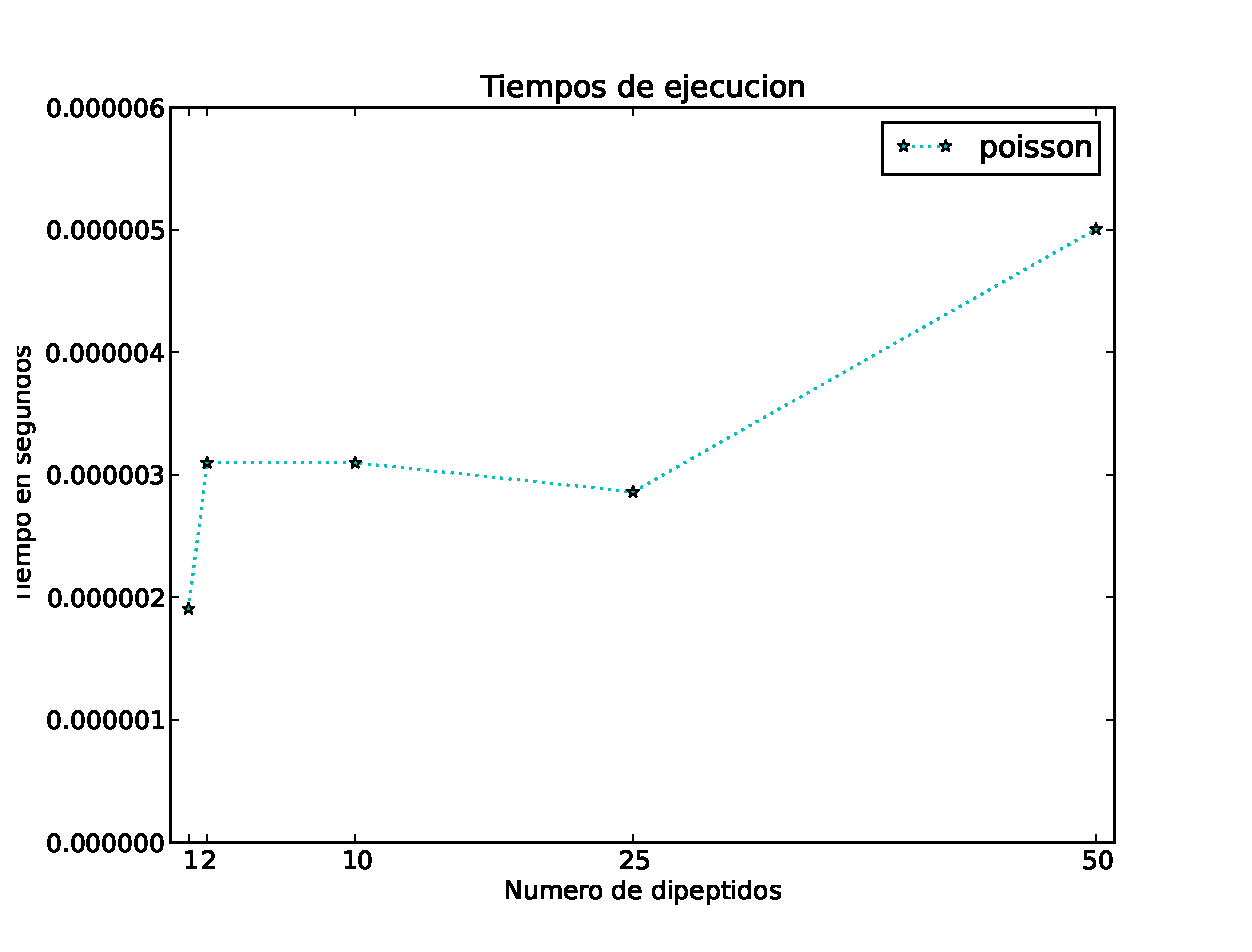
\includegraphics[width=0.75\textwidth]{images/tiempo_ejecucion.eps}
\caption{Tiempos de ejecucion del algoritmo}
\label{fig:1}
\end{center}
\end{figure}

\\
\\
El Ap�ndice 1 incluye tambi�n los nombres de los archivos con los algoritmos implementados para obtener los datos de la m�quina y los tiempos de ejecuci�n.


%++++++++++++++++++++++++++++++++++++++++++++++++++++++++++++++++++++++++++++++
\section{Resultados obtenidos}
\label{3:sec:3}

Las siguientes tablas y gr�ficos representan los resultados obtenidos en el experimento y adem�s una comparaci�n con resultados reales observados y experimentos anteriores a la aplicaci�n de la distribuci�n de Poisson. 
V�ase el Cuadro \ref {tabla2} y la Figura \ref {fig:2}

%------------------------------------------------------------------------------
\begin{figure}[!th]
\begin{center}
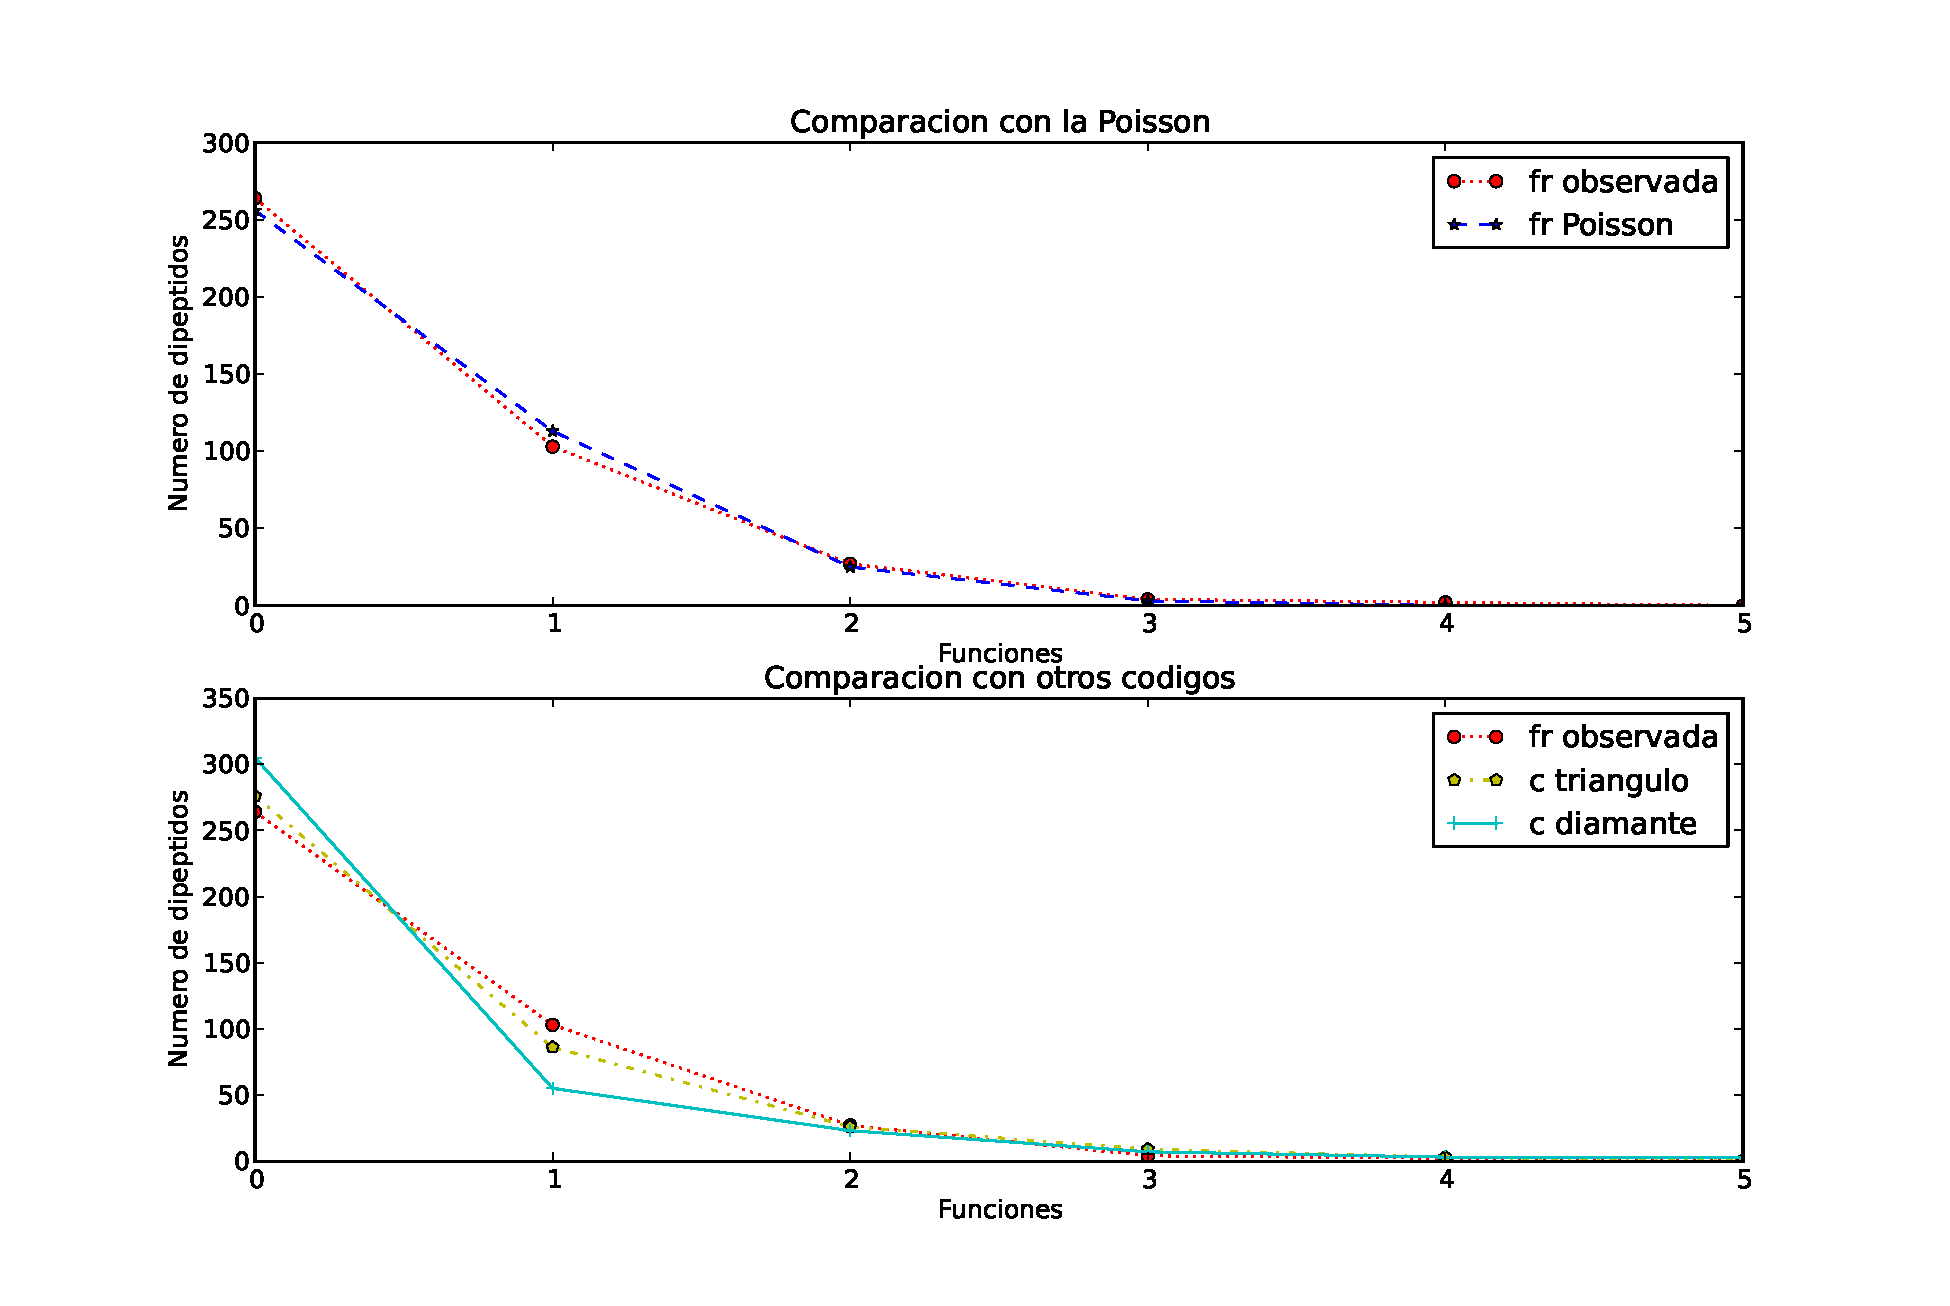
\includegraphics[width=0.75\textwidth]{images/comparacion.eps}
\caption{Comparacion Poisson-C Diamante-C Triangulo}
\label{fig:2}
\end{center}
\end{figure}
%------------------------------------------------------------------------------


%------------------------------------------------------------------------------
\begin{table}[!ht]
\begin{center}
\begin{tabular}{llll}
N dipeptidos & Frec. observada & P(x) (Poisson) & Frecuencia Total 400xP(x) \\
\hline
0 & 264 & 0.6424283410 & 256.9713363872\\
1 & 102 & 0.2842745409 & 113.7098163514\\
2 & 27 & 0.0628957422 & 25.1582968677\\
3 & 4 & 0.0092771220 & 3.7108487880\\
4 & 2 & 0.0010262816 & 0.4105126472\\
5 & 0 & 0.0000908259 & 0.0363303693\\
6 & 0 & 0.0000066984 & 0.0026793647\\
7 & 0 & 0.000004234 & 0.0001693741\\
8 & 0 & 0.000000234 & 0.0000093685

\end{tabular}
\\
\\
\\
\\
\\

\begin{tabular}{llll}
N dipeptidos & Frec. observada & Codigo Triangulo & Codigo Diamante\\
\hline
0 & 264 & 276 & 305\\
1 & 102 & 86 & 55\\
2 & 27 & 26 & 23\\
3 & 4 & 9 & 7\\
4 & 2 & 3 & 3\\
5 & 0 & 0 & 3\\
6 & 0 & 0 & 2\\
7 & 0 & 0 & 0\\
8 & 0 & 0 & 2

\end{tabular}
\end{center}
\caption{Comparacion}
\label{tabla2}
\end{table}
%------------------------------------------------------------------------------

%++++++++++++++++++++++++++++++++++++++++++++++++++++++++++++++++++++++++++++++
\section{An�lisis de los resultados}
\label{3:sec:4}

Haciendo un an�lisis detallado de los datos que muestran las tablas, puede observarse que la distribuci�n de Poisson es la que describe en mejor medida el experimento. 
\\
Es claro que al comparar las gr�ficas, la funci�n que representa la distribuci�n de Poisson se acerca mucho m�s a los datos reales observados.
\\
Sin embargo, los experimentos anteriores (Codigo Diamante y Codigo Triangulo) son algo menos acertados.
\\
Se infiere de la observaci�n que a medida que aumenta el n�mero de dip�ptidos, es menos probable encontrar casillas que los contengan, es decir, existen muchas m�s casillas con una cantidad peque�a de dip�ptidos que casillas con grandes cantidades. De hecho, se ha elegido como 'n' = 8 porque a partir de esta cantidad, la probabilidad de que las casillas est� vac�as es casi total. 
\\
Este hecho podr�a ser �til en diferentes campos de la biolog�a o la medicina, entre otros.



%%%%%%%%%%%%%%%%%%%%%%%%%%%%%%%%%%%%%%%%%%%%%%%%%%%%%%%%%%%%%%%%%%%%%%%%%%%%%%%
\chapter{Conclusiones}
\label{chapter:conclusiones}

%%%%%%%%%%%%%%%%%%%%%%%%%%%%%%%%%%%%%%%%%%%%%%%%%%%%%%%%%%%%%%%%%%%%%%%%%%%%%
% Chapter 4: Conclusiones y Trabajos Futuros 
%%%%%%%%%%%%%%%%%%%%%%%%%%%%%%%%%%%%%%%%%%%%%%%%%%%%%%%%%%%%%%%%%%%%%%%%%%%%%%%

%Como conclusión principal puede decirse que implementando un algoritmo que representa el problema que se quiere resolver, se ahorra tiempo al obtener los resultados, y además éstos pueden ser respresentados en gráficas y tablas para realizar comparaciones con otros experimentos.\\

%Además, el algoritmo no es válido únicamente para el ejemplo en el que se centra el informe, ya que al describir la misma función, simplemente cambiando los datos de entrada puede adaptarse a gran variedad de experimentos con las mismas carácterísticas, con lo cual abarca un campo de estudio mucho más amplio.\\

%Respecto a los propios datos, se llega a la conclusión de  que una distribución de Poisson describe mucho mejor el experimento que algunas de las técnicas más antiguas llevadas a cabo como pueden ser los mencionados 'Código Diamante' y 'Código Triángulo' , ya que los datos obtenidos se aproximan con más exactitud a los reales observados. Este hecho asegura cierta confianza en posibles futuras aplicaciones del experimento en diferentes campos.

%\\

Como conclusion principal puede decirse que implementando un algoritmo que representa el problema que se quiere resolver, se ahorra tiempmo al obtener los resultados y ademas estos pueden ser representados en graficas y tablas para realizar comparaciones con otros experimentos\\
Ademas, el algoritmo no es valido unicamente para el ejemplo en el que se centra el informe, ya que al describir la misma funcion, simplemente cambiando lso datos de entrada puede adaptarse a gran variedad de experimentos con las mismas caracteristicas, con lo cual abarca un campo de estudio mucho mas amplio.\\
Respecto a los propios datos, se llega a la conclusion de que una distribucion de Poisson descrie mucho mejor el eperimento que algunas de las tecnicas mas antiguas llevadas a cabo como pueden ser los mencionados 'Codigo Diamante'  y 'Codigo Triangulo' , ya que los datos obtenidos se aproximan con mas exactitud a los reales observados. Este hecho asegura cierta confianza en posibles futuras aplicaciones del experimento en diferentes campos.

%%%%%%%%%%%%%%%%%%%%%%%%%%%%%%%%%%%%%%%%%%%%%%%%%%%%%%%%%%%%%%%%%%%%%%%%%%%%%%%

%%%%%%%%%%%%%%%%%%%%%%%%%%%%%%%%%%%%%%%%%%%%%%%%%%%%%%%%%%%%%%%%%%%%%%%%%%%%%%%
\newpage{\pagestyle{empty}\cleardoublepage}
\thispagestyle{empty}
\begin{appendix}

\chapter{Archivos adjuntos}
\label{appendix:1}

\section{Algoritmos utilizados}
\label{Apendice1:XXX}
\\
A continuacion se muestran los nombres de los ficheros adjuntos a este informe que han sido utilizados para implementar las funciones y crear las tablas y graficos.\\
%\begin{center}
%\begin{footnotesize}
%\begin{verbatim}
\begin{enumerate}
\item poisson.py : Algoritmo en Python en el que se ha desarrollado la funcion principal
\item informacion.py : Algoritmo en Python que proporciona la informacion de la maquina
\item tiempos.py : Algoritmo en Python que calcula el tiempo que tarda la maquina en ejecutar Poisson.py.
\item graf tiempo.py : Algoritmo en python que genera la grafica del tiempo que de tiempos.py
\item tablas.tex : Archivo LaTeX que genera las tablas de datos de comparacion de la Poisson\\
\end{enumerate}
%\end{footnotesize}
%\end{center}

%\section{Algoritmo YYY}
%\label{Apendice1:YYY}

%\begin{center}
%\begin{footnotesize}
%\begin{verbatim}


%\end{footnotesize}
%\end{center}


%\chapter{T�tulo del Ap�ndice 2}
%label{appendix:2}

%\section{Otro apendice: Seccion 1}
\label{Apendice2:label}

\begin{center}
\begin{footnotesize}

\begin{verbatim}
Texto
\end{verbatim}

\end{footnotesize}
\end{center}

\section{Otro apendice: Seccion 2}
\label{Apendice2:label2}

\begin{center}
\begin{footnotesize}

\begin{verbatim}
Texto
\end{verbatim}


\end{footnotesize}
\end{center}


\end{appendix}

%%%%%%%%%%%%%%%%%%%%%%%%%%%%%%%%%%%%%%%%%%%%%%%%%%%%%%%%%%%%%%%%%%%%%%%%%%%%%%%
\addcontentsline{toc}{chapter}{Bibliograf�a}
\bibliographystyle{plain}
\begin{thebibliography}{11}
\bibitem{fundamentos} Fundamentos de Probabilidad en Estadistica. G.Alonso. J.Oca�a. C.M.Cuadras.
\bibitem{librodos} Estadistica Teorica y Aplicada. Andres Nortes Checa.
\bibitem{web} http://www.itch.edu.mx/academic/industrial/sabaticorita/private/05Distr%20Poisson.htm
\bibitem{webdos} http://www.aulafacil.com/CursoEstadistica/Lecc-29-est.htm
\end{thebibliography}

\bibliography{bib/references}
\nocite{*}

%%%%%%%%%%%%%%%%%%%%%%%%%%%%%%%%%%%%%%%%%%%%%%%%%%%%%%%%%%%%%%%%%%%%%%%%%%%%%%%
\footnote{Facultad de Matem�ticas. T�cnicas Eperimentales. Universidad de La Laguna}
\end{document}
